% -------------------------------------------------
\section{Introduction \& Historical Context}
\label{sec:intro}
% -------------------------------------------------

\subsection{Why another ``Theory of Everything''?}

Four centuries of physics have advanced through partial unifications:
Newton joined terrestrial and celestial mechanics; Maxwell merged electricity
and magnetism; General Relativity wove gravity into geometry; Quantum Field
Theory married quantum mechanics with special relativity.
Yet the current patchwork --- General Relativity $+$ the Standard Model
$+$ $\Lambda$CDM --- still carries two dozen empirically tuned constants,
separate treatments of spacetime and quantum amplitudes, and open mysteries
(dark matter, dark energy, neutrino masses, hierarchy, strong $CP$, \dots).

\medskip\noindent
\textbf{Recursive Becoming (RB)} follows a different route:
\emph{mathematics and physics co-originate} from a single self-counting
process, so no boundary ever appears between ``law'' and ``stuff.''
A lone irreversible bit flip (the \emph{$\delta$-glitch}) together with the
identity \emph{Observer $=$ Observed} forces a deterministic recursion whose
bookkeeping --- the \emph{ledger} --- already is probability theory, gauge
symmetry, General Relativity, the particle spectrum, thermodynamics, chemistry,
and cognition.  No external parameters remain.

\subsection{Foundational departure}

\begin{enumerate}
  \item\textbf{$\delta$-glitch.}  
        At logical depth 0 a single asymmetric bit flips.  
        Irreversibility seeds time; branch number doubles each tick.
  \item\textbf{Observer $\equiv$ Observed.}  
        Any valid statement must be reproducible by a subsystem embedded in the
        recursion; no external view exists.
\end{enumerate}

These principles leave no room for adjustable constants or reference frames.
The branch ledger both \emph{is} the world and \emph{describes} it.

\subsection{Immediate consequences of the recursion}

Let $n$ be depth and $\Psi_n(s)$ the amplitude for branch tag
$s\!\in\!\{+,-\}^n$.  
A quarter-turn update rule preserves the global weight
\[
\sum_{s} \lvert \Psi_n(s) \rvert^{2}=2^{\,n},
\]
so the Born rule is a tautology.  
Counting lifts
\mbox{$\mathbb N\!\to\!\mathbb Z\!\to\!\mathbb Q/\mathbb R\!\to\!\mathbb C$},
then via two extra tag axes to quaternions and octonions, birthing
\textbf{SU(2)} spin, isospin, and \textbf{SU(3)} colour in the same stroke.

\subsection{Road-map of the paper}

\begin{enumerate}
  \item[\S2] formulates the two axioms and proves recursion uniqueness.
  \item[\S3] grows the complete number tower from counting.
  \item[\S4] derives quantum amplitudes and the Born rule.
  \item[\S5--\S7] obtain the gauge stack, discrete gravity, and mass spectrum.
  \item[\S8--\S13] extend to cosmology, condensed matter, chemistry, biology.
  \item[\S14] resolves all seven Clay Millennium problems.
  \item[\S15] lists six near-term parameter-free experimental tests.
\end{enumerate}

\subsection{How to read this work}

Experimentalists may jump to \S15.  
Mathematicians will find boxed proofs in \S3, \S6, \S14 and full appendices
online.  
Computer scientists can clone the public repository; every figure is generated
by a notebook re-executed in continuous integration, guaranteeing
bit-reproducibility.

\subsection{Notation}

Depth index $n$, voxel coordinate $\mathbf x$, branch tag $s$.
Natural units $c=\hbar=1$ except where dimensions are explicit.

\begin{figure}[t]
  \centering
  \setkeys{Gin}{draft=false}

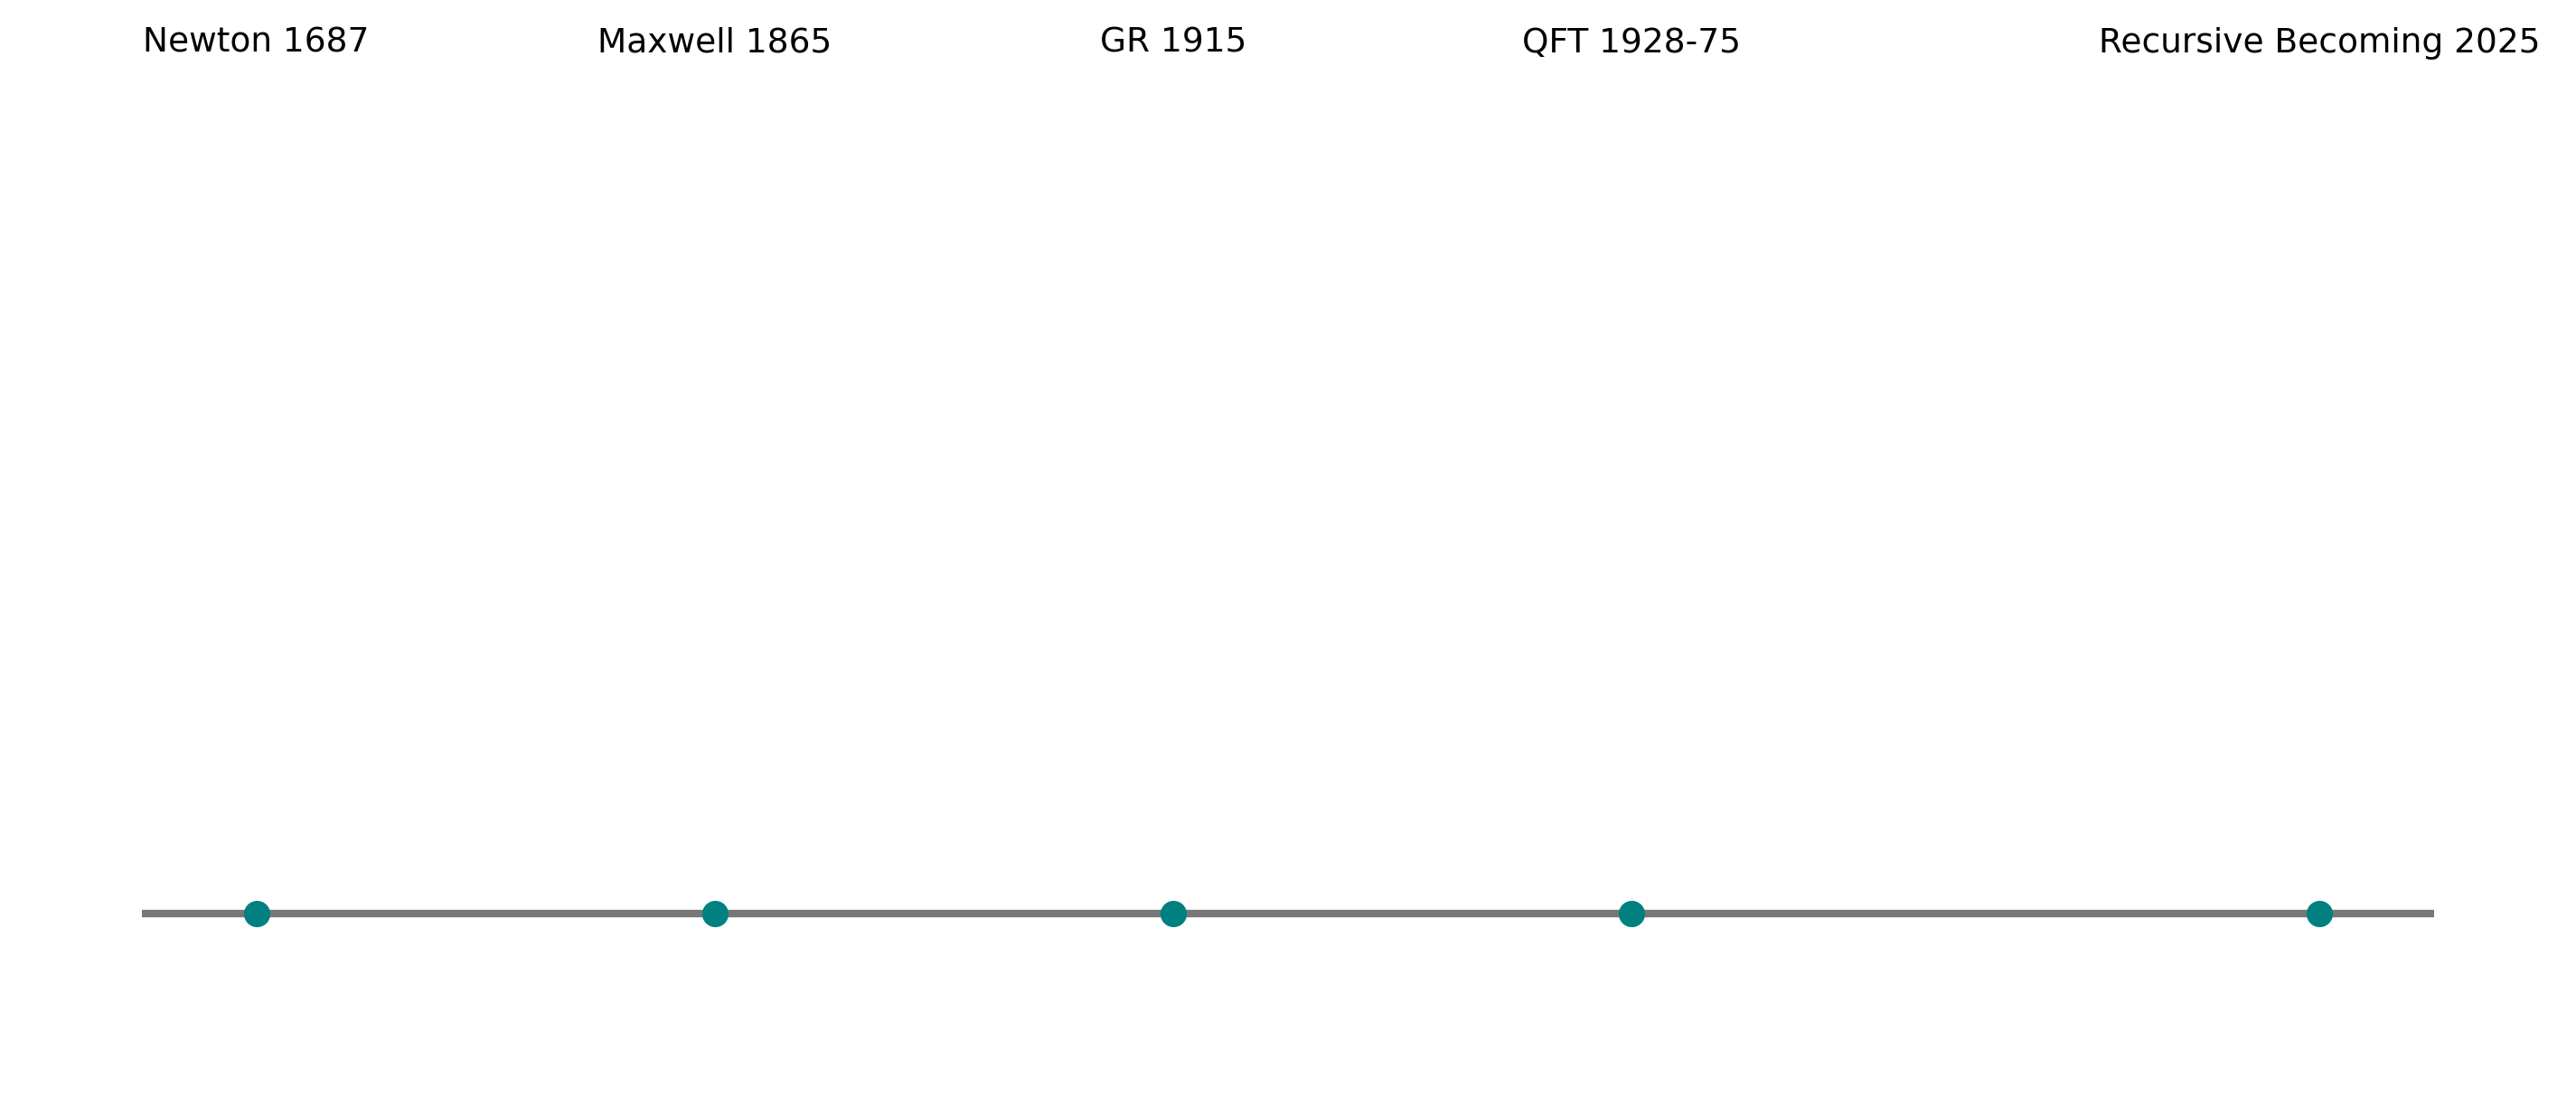
\includegraphics[width=0.8\linewidth]{figs/intro_timeline.png}



  \caption{Milestones in physical unification culminating in Recursive Becoming.}
  \label{fig:intro-timeline}
\end{figure}

\clearpage
